\documentclass[12pt]{article}
\usepackage[none]{hyphenat}
\usepackage{amsmath}
\usepackage{graphicx}
\title{\textbf{TOP DOWN PARSER BUILT IN JAVA}}
\author{Akash Kulkarni\\4JC11CS006\and Anurag Kakati\\4JC11CS015}
\date{\today}
\renewcommand{\familydefault}{\sfdefault}
\begin{document}
\maketitle
\section{Abstract}
A new approach to designing system level softwares such as parsers using a high level programming language, namely Java, is presented in this paper. Parsing or syntactic analysis is the process of analysing a string of symbols, either in natural language or in computer languages, according to the rules of a formal grammar. A parser is a software component that takes input data and builds a parse tree, abstract syntax tree or other hierarchical structure – giving a structural representation of the input, checking for correct syntax in the process. The parser is often preceded by a separate lexical analyser, which creates tokens from the sequence of input characters. Top-down parsing is a parsing strategy where one first looks at the highest level of the parse tree and works down the parse tree by using the rewriting rules of a formal grammar. An LL parser is a type of parser that does top-down parsing by applying each production rule to the incoming symbols, working from the left-most symbol yielded on a production rule and then proceeding to the next production rule for each non-terminal symbol encountered. The parser implemented is an LL(1) parser where the (1) signifies the parser reads ahead one token at a time.
\section{Top Down Parsers}
An example for a typical top down parser is a Recursive-Descent parser. A recursive-descent parsing program consists of a set of procedures for each non-terminal. Execution begins with the procedure for the start symbol, which halts and announces success if its procedure body scans the entire input string. The limitations of a recursive-descent parser are:
\begin{itemize}
\item A left-recursive grammar can cause a recursive-descent parser to go into an infinite loop.
\item A recursive-descent parser has exponential time complexity.
\end{itemize}
To eliminate the problem of exponential time complexity, LL(1) parsers were introduced.
\subsection{First and Follow}
The construction of top-down parser is aided by two functions, FIRST and FOLLOW, associated with a grammar G.\\
	Define \textit{FIRST(}$\alpha$\textit{)}, where $\alpha$ is any string of grammar symbols, to be the set of terminals that begin strings derived from $\alpha$. If $\alpha$ $\overset{\ast}{\Rightarrow}$ $\epsilon$, then $\epsilon$ is also in FIRST($\alpha$).
To compute FIRST($X$) for all grammar symbols $X$, apply the following rules until no more terminals or $\epsilon$ can be added to any FIRST set.
\begin{enumerate}
\item If $X$ is a terminal, then FIRST($X$) = \{\textit X\}
\item If $X$ is a nonterminal and $X$ $\rightarrow$ $Y_1$$Y_2$ $\cdots$ $Y_k$ is a production for some $k \ge 1$, then place $a$ in FIRST($X$) if for some $i$, $a$ is in FIRST($\textit{Y}_i$), and $\epsilon$ is in all of FIRST($\textit{Y}_1$),$\dots$,FIRST($Y_{i-1}$); that is, $Y_1$$\cdots$$Y_{i-1}$ $\overset{\ast}{\Rightarrow}$ $\epsilon$. If $\epsilon$ is in FIRST($Y$) for all $j=1,2,\dots,k,$ then add $\epsilon$ to FIRST($X$).
\item If $X \rightarrow \epsilon$ is a production, then add $\epsilon$ to FIRST($X$)
\end{enumerate}
Define FOLLOW($A$), for a non-terminal $A$, to be the set of terminals $a$ that can appear immideately to the right of $A$ in some sentential form; that is, the set of terminals $a$ such that there exists a derivation of the form $S \overset{\ast}{\Rightarrow} \alpha Aa\beta$, for some $\alpha$ and $\beta$. \\
To compute FOLLOW($A$) for all nonterminals $A$, apply the following rules until nothing can be added to any FOLLOW set.
\begin{enumerate}
\item Place $\$$ in FOLLOW($S$), where $S$ is the start symbol, and \$ is the input right end marker.
\item If there is a production $A \rightarrow \alpha B\beta$, then everything in FIRST($\beta$) except $\epsilon$ is in FOLLOW($B$)
\item If there is a production $A \rightarrow \alpha B$, or a production $A \rightarrow \alpha B\beta$, where FIRST($\beta$) contains $\epsilon$, then everything in FOLLOW($A$) is in FOLLOW($B$).
\end{enumerate} 
\subsection{Parsing via construction of parsing table}
\textbf{Algorithm} : Construction of parsing table. \\
\\
\textbf{INPUT} : Grammar $G$ \\
\\
\textbf{OUTPUT} : Parsing table $M$ \\
\\
\textbf{METHOD} : For each production $A \rightarrow \alpha$ of the grammar, do the following:
\begin{enumerate}
\item For each terminal $\alpha$ in FIRST{$A$}, add $A \rightarrow \alpha$ to $M[A, a]$.
\item If $\epsilon$ is in FIRST($\alpha$), then for each terminal $b$ in FOLLOW($A$), add $A \rightarrow \alpha$ to $M[A,b]$. If $\epsilon$ is in FIRST($\alpha$) and \$ is in FOLLOW($A$), add $A \rightarrow \alpha$ to $M[A,\$]$ as well.  
\end{enumerate}
Algorithm for non-recursive predictive parsing is given below: \\
\\
\textbf{Algorithm} : Table-driven predictive parsing.\\
\\
\textbf{INPUT} : A string $w$ and a parsing table $M$ for grammar $G$. \\
\\
\textbf{OUTPUT} : If $w$ is in $L(G)$, a leftmost derivation of $w$; otherwise, an error indication.\\
\\
\textbf{METHOD} : Initially, the parser is in a configuration with $w\$$ in the input buffer and the start symbol $S$ of $G$ on top of the stack, above \$. \\
\\
\indent {set \textit{ip} to point to the first symbol of $w$}; \\
\indent {set $X$ to the top stack symbol}; \\
\indent {\textbf{while} ($X \ne \$$) \{} \\
\indent\indent {\textbf{if}( $X \ is \ a$ ) pop the stack and advance ip}; \\
\indent\indent {\textbf{else if}( $X$ is a terminal ) $error()$}; \\
\indent\indent {\textbf{else if}( $M[X,a]$ is an error entry ) $error()$}; \\
\indent\indent {\textbf{else if}( $M[X,a] = X \rightarrow Y_{1}Y_{2}\cdots Y_{k}$ )\{}\\
\indent\indent\indent {output production $X \rightarrow Y_{1}Y_{2}\cdots Y_{k}$};\\
\indent\indent\indent {pop the stack}; \\
\indent\indent\indent {push $Y_{k},Y_{k-1},\dots,Y_{1}$ onto the stack, with $Y_{1}$ on top};\\
\indent\indent \} \\
\indent\indent {set $X$ to top stack symbol};\\
\indent \} \\
\\
The parser implemented follows the above mentioned algorithms. First, Follow, and the Parsing table implementations mainly use the dictionary data-type available in Java. The parsing action implementation uses the traditional stack data structure for storing the non-terminals that are encountered during parsing. The dictionary data-type is an extended version of hashing and hence the efficiency of the retrieval operation from those data-types is in $O(n)$. 
\section{Simulation Results}
\begin{figure}[ht!]
\centering
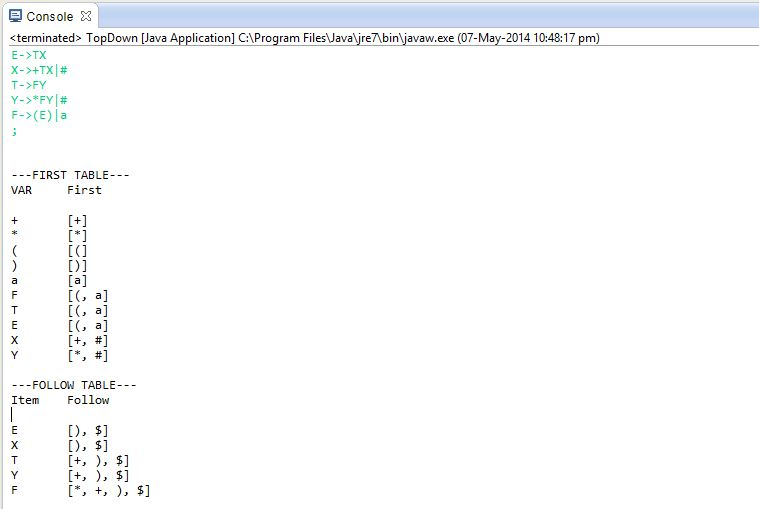
\includegraphics[width=100mm]{TDP1.jpg}
\end{figure}
\begin{figure}[ht!]
\centering
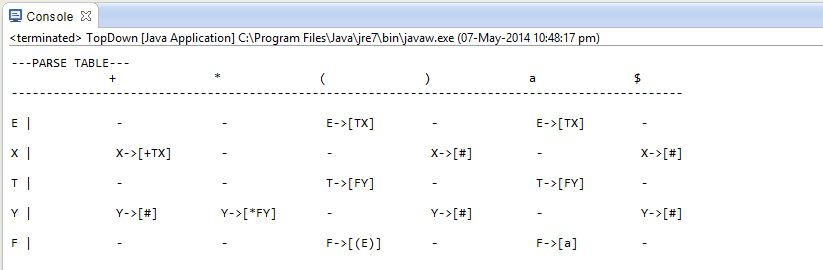
\includegraphics[width=100mm]{TDP2.jpg}
\end{figure}
\begin{figure}[ht!]
\centering
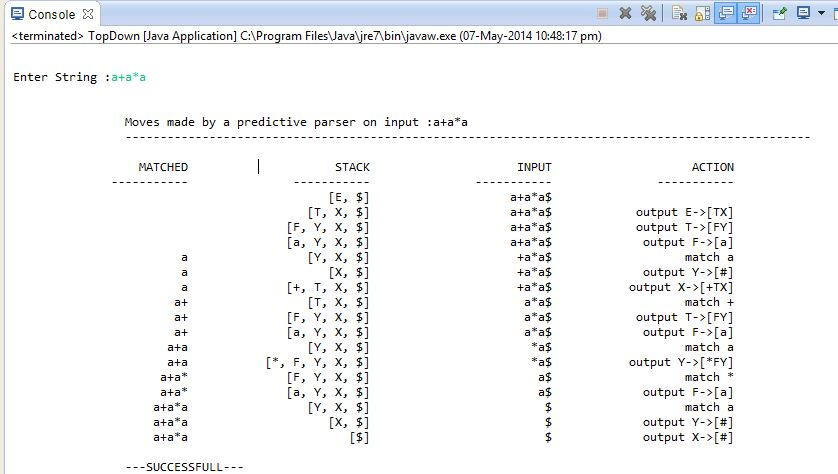
\includegraphics[width=100mm]{TDP3.jpg}
\end{figure}
\section{Conclusion}
The advantage of using a high level language like Java is clearly enumerated by the design and execution of the program. It is easier to design the parser in Java than most other programming languages and advanced concepts like memoization and advanced datatypes like ArrayLists make for a more efficient parsing of input data.
\section{References}
\begin{enumerate}
\item Wikipedia
\item Compilers Principles, Techniques, and Tools - Alfred V Aho, Monica S Lam, Ravi Sethi, Jeffery D Ullman
\item HeadFirst Java
\end{enumerate}
\end{document}
